\begin{frame}{Applications of Protein Language Models}
    \begin{tikzpicture}
        % Nodes for Applications
        \node (a1) [draw, rounded corners, fill=blue!20, text centered, minimum width=3cm, minimum height=1cm] at (0,-2) {Protein Structure Prediction};
        \node (a2) [draw, rounded corners, fill=green!20, text centered, minimum width=3cm, minimum height=1cm] at (6,0) {Drug Discovery};
        \node (a3) [draw, rounded corners, fill=orange!20, text centered, minimum width=3cm, minimum height=1cm] at (6,-2) {Disease Understanding};
        \node (a4) [draw, rounded corners, fill=purple!20, text centered, minimum width=3cm, minimum height=1cm] at (6,-4) {Synthetic Biology};

        % Arrows between the applications
        \pause
        \draw[->, thick] (a1) -- (a2);
        \draw[->, thick] (a1) -- (a3);
        \draw[->, thick] (a1) -- (a4);
        
        % Add small icons for each application
        \node at (-2,-1.3) {
\includegraphics[width=0.8cm]{images/protein.PNG}}; % Protein structure icon
        \node at (7,0.7) {
\includegraphics[width=0.8cm]{images/pill.PNG}}; % Drug discovery icon
        \node at (7.5,-1.3) {
\includegraphics[width=0.8cm]{images/microscope.PNG}}; % Disease icon
        \node at (7,-3.3) {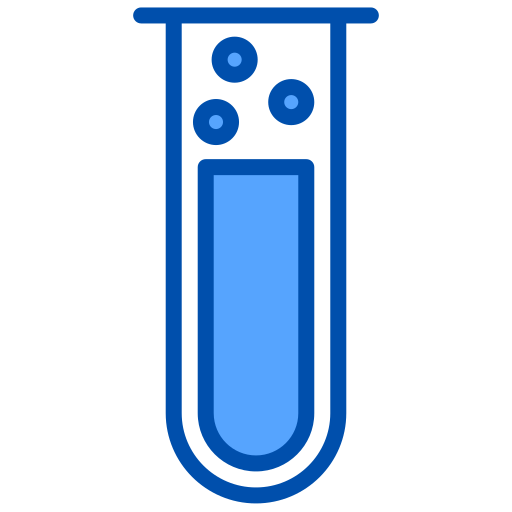
\includegraphics[width=0.8cm]{images/testtube.PNG}}; % Synthetic biology icon
    \end{tikzpicture}
\end{frame}
